\section{Úrovně řízení výroby a jejich funkce. Zařazení komponent do jednotlivých vrstev a možnosti jejich propojení. Způsob řízení výroby (centralizované a distribuované). Toky dat (informací) v systému a jejich popis. Vlastnosti a možnosti nadřazených výrobních systémů (MES, ERP).}
\subsection{Struktura řídícího systému výrobního podniku}
\begin{figure}[h]
    \begin{center}
        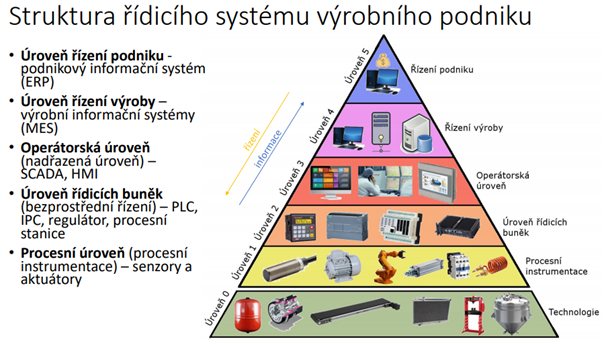
\includegraphics[width=\textwidth]{img/rizeni.png}
    \end{center}
\end{figure}

\subsubsection*{Úrověň řízení podniku - ERP}
\begin{itemize}
    \item Podnikový informační systém - ERP (= Enterprise Resource Planning).
    \item Zařizuje nákup, logistiku, distribuci, účetnictví, fakturace.
\end{itemize}

\subsubsection*{Úroveň řízení výroby - MES}
\begin{itemize}
    \item Výrobní informační systém - MES (= Matufacturing Execution System).
    \item Shromažďuje data o výrobě a na základě těchto dat posílá příkazy do jednotlivých částí výroby.
    \item Věnuje se například správě výrobních zdrojů, plánováním výroby, řízení výroby, sběr dat, kontrola jakosti, výkonnostní analýzy.
\end{itemize}

\subsubsection*{Operátorská úroveň - SCADA, HMI}
\begin{itemize}
    \item Systém SCADA (= Supervisory Control And Data Acquisition), HMI (= Human Machine Interface) - nadřazená úroveň PLC.
    \item SCADA je vzdálený monitorovací systém - například velín. Jedná se o software monitorující průmyslová a technická zařízení, jejich procesy a umožňuje vzdálené ovládání.
    \item HMI je dotyková obrazovka, umožňující ovládání a monitorování procesu přímo u daného zařízení.
    \item Lidská činnost - definování procesu, hlídání chybových hlášení, správa atp.
\end{itemize}

\subsubsection*{Úroveň řídícíh buněk}
\begin{itemize}
    \item Bezprostřední řízení procesů pomocí PLC, IPC, regulátory, procesní stanice.
    \item Systémy přímo napojené na výrobní prostředek, spravující jeho sledování a nastavování.
\end{itemize}

\subsubsection*{Procesní úroveň}
\begin{itemize}
    \item Snímače, akční členy (aktuátory), motory, roboti.
    \item Snímače získávají data z výrobního procesu. Akční členy tyto procesy nějakým způsobem ovlivňují.
\end{itemize}

\subsubsection*{Technologie}
\begin{itemize}
    \item Elektrické přostředky, tepelné zařízení, dopravníkový pás, převodovky,...
\end{itemize}

\subsection{Možnosti propojení úrovní řízení}
\begin{itemize}
    \item ERP - MES = komunikace pomocí ethernetu.
    \item SCADA - PLC = komunikace pomocí ethernetu - například standard OPC UA.
    \item PLC - HMI = komunikace pomocí sériové komunikace, ethernet. Například Modbus TCP, Ethernet/IP, ProfiNET.
    \item PLC - Snímače = propojeny elektronicky (pomocí digitálních/analogových vstupů/výstupů - proudové smyčky 4-20mA), sběrnicí - IO-Link, AS-Interface, Profibus.
\end{itemize}

\subsection{Centralizované a distribuované řízení výroby}
\subsubsection*{Distribuované - DCS}
\begin{itemize}
    \item DCS = Distributed Control System.
    \item Každá řídící komponenta má na starost svou dílčí oblast, která je do jisté míry autonomní - například PLC.
    \item Tyto komponenty komunikují mezi sebou, případně s nadřazeným systémem, který je ovládá jako celek.
\end{itemize}

\subsubsection*{Centralizované}
\begin{itemize}
    \item Řízení z jednoho organizačního ústředí = jeden řídící komponent, kde se vyhodnocuje logika pro řízení všech procesů.
\end{itemize}

\begin{figure}[h]
    \begin{center}
        \includegraphics[scale = 1]{img/picture2.png}
    \end{center}
\end{figure}

\subsection{Toky dat a druhy řízení}
V principu ERP zapisuje do MES požadavky na výrobu, MES podle požadavku nastavuje výrobní prostředky. Z výrobních prostředků se vrací informace o jejich stavu (výkonnost, opotřebení, spotřeba materiálu), které MES nějakým způsobem zaobaluje, aby tyto informace byly „použitelné pro business“.

\begin{figure}[h]
    \begin{center}
        \includegraphics[scale = 1]{img/picture3.png}
    \end{center}
\end{figure}


\subsection{Vlastnosti a možnosti nadřazených výrobních systémů (MES,ERP)}
\subsubsection*{ERP}
\begin{itemize}
    \item Slouží k řízení podniku, obchodní část systémů, logistika, distribuce, správa majetku, faktury, učetnictví,\dots
    \item Výhody:\begin{itemize}
              \item Zefektivnění a zrychlení podnikových procesů
              \item Centralizace a vyčištění dat, snížení chybovosti
              \item Méně byrokracie
              \item Vyšší bezpečnost
          \end{itemize}
    \item Funkce: \begin{itemize}
              \item Vyřizování objednávek
              \item Nákup materiálu
              \item Zajišťování lidských zdrojů
              \item Výpočet ziskovosti
              \item Prodej a distribuce produktů
          \end{itemize}
\end{itemize}

\subsection{MES}
\begin{itemize}
    \item Informační a řídící systém podporující efektivní provádění výrobních operací.
    \item Sbírá aktuální a přesná data, navádí a spouští aktivity v závodě a podává informace "výš".
    \item Funkce: \begin{itemize}
              \item Správa výrobních zdrojů a postupů
              \item Plánování výroby a řízení ze strany dispečera
              \item Jakostní a výkonnostní analýzy
              \item Sběr dat
          \end{itemize}
    \item Spolupráce s ERP: \begin{itemize}
              \item Nastavení výroby dle požadavků ERP - množství, kvalita, receptura = možnosti výroby.
          \end{itemize}
\end{itemize}

\section{Standardní rozhraní průmyslových signálů - typy, obvodové provedení, vlastnosti a použití. Logika digitálních signálů. Zpracování analogové veličiny. Standardizace a destandardizace. Senzory - popis, typy a jejich použití. Možnosti zapojení
  snímačů do systému.}

\subsection{Standardní rozhraní průmyslových signálů - typy, obvodové provedení, vlastnosti a použití}
Rozhraní je fyzicky tvořeno buď tranzistorovou logikou, nebo pomocí relé. Používá se několik napěťových a proudových úrovní.
\subsubsection*{Rozhraní - spojité}
\begin{itemize}
    \item Průmyslová logika 24 VDC: \begin{itemize}
              \item Logická "0" \dots -30 - 5 VDC
              \item Logická "1" \dots 13 - 30 VDC
          \end{itemize}
    \item Značení: \begin{itemize}
              \item NO - Normally Open (pokud není energizován, je rozepnut) = spínací kontakt
              \item NC - Normally Closed (pokud není energizován, je sepnut) = rozpínací kontakt
              \item FO - Fail Open (Při poruše zůstane rozepnut)
              \item FC - Fail Close (Při poruše zůstane sepnut)
              \item FL - Fail Last (Při poruše zůstane v poslední poloze)
          \end{itemize}
    \item Fyzicky jsou vstupy realizovány jako: \begin{itemize}
              \item HTL (High Treshold Logic) - push-pull - využity dva tranzistory na výstupu, dosah až 100 m, pro prostředí s větším rušením - vhodné pro průmysl
              \item TTL (Transistor Transistor Logic) - logická "1" je pouze 2-5 VDC, využitá se u RS422 (Kroucená dvoulinka, dosah až kilometr), obecně napájeno z nižších napětí (5V, 1,7V), používá se na DPS.
              \item Open Collector - Pouze 1 tranzistor, dosah 10 m. Logická "1": 2-30 VDC, Logická "0": 0 - 0.5 VDC.
          \end{itemize}
\end{itemize}

\subsubsection*{Obvodové provedení}
\begin{itemize}
    \item Sink a Source - Udává, na keré straně zdroje se spíná
    \item Sink se připojuje se zemí
    \item Source se spojuje s Ucc
    \item Pro sourcing snímač se použije sinking vstup a naopak
\end{itemize}

\begin{figure}[h]
    \begin{center}
        \includegraphics[scale = 1]{img/picture5.png}
    \end{center}
\end{figure}

\subsubsection*{Zpracování analogových veličin}
\begin{itemize}
    \item Napětí - rozsah: 0 až 10 V, dochází rušení z ostatních vodičů díky indukci, napětí s delkou vedení klesá.
    \item Proud - rozsah 4-20 mA (0-20 mA), tzv. proudová smyčka, odolnější proti rušení, lze detekovat poruchu (0 mA) a ze smyčky lze zařízení i napájet.
    \item Zapojení může být 2-vodičové (např. měření odporu PT100), 3-vodičové (např. měření polohy (potenciometr)), 4-vodičové (snímač s vlastním napájením + proudová smyčka)
\end{itemize}

\begin{figure}[h]
    \begin{center}
        \includegraphics[scale = 1]{img/picture4.png}
    \end{center}
\end{figure}

\subsubsection*{Měřící rozsahy}
\begin{itemize}
    \item Bipolární (kladné i záporné), Unipolární (pouze kladné)
\end{itemize}

\subsection{Standardizace a destandardizace}
\subsubsection*{Standardizace}
\begin{itemize}
    \item Jedná se o převod elektrické veličiny na reálné číslo v příslušných inženýrských jednotkách, které se budou nacházet v zadaných mezích.
    \item Standardizovaná hodnota lze dále uživatelsky využívat - např. zobrazení na operátorském panelu.
    \item x = naměřená hodnota
    \item MAX,MIN = vstupní analogová proměnná (např. teplota)
    \item k1 = min hodnota převodníku
    \item k2 = max hodnota převodníku
\end{itemize}

\begin{figure}[h]
    \begin{center}
        \includegraphics[scale = 1]{img/picture6.png}
    \end{center}
\end{figure}

\subsubsection*{Destandardizace}
\begin{itemize}
    \item Opačný převod jako standardizace.
    \item Převod reálného čísla na elektrickou veličinu.
    \item Využívá se k řízení pomocí akčních regulačních členů.
\end{itemize}

\subsection{Senzory}

\subsubsection*{Čidlo}
\begin{itemize}
    \item Převodník mechanické/tepelné/elektrické/magnetické/... energie na elektrickou.
    \item Jednoduché a rychlé zpracování analogové i digitální.
    \item Rychle měření a spolehlivý přenos.
\end{itemize}

\subsubsection*{Inteligentní snímač}
\begin{itemize}
    \item Měří a rovnou i zpracovává měřenou veličinu.
    \item Obsahuje procesor, má standardní výstup nebo komunikační sběrnici (protokol).
    \item Skládá se z modulu pro měření, vyhodnocení a komunikaci.
\end{itemize}

\subsubsection*{Rozdělení}
\begin{itemize}
    \item Aktivní/pasivní:\begin{itemize}
              \item Aktivní - Chová se jako zdroj elektrické energie
              \item Pasivní - Potřebuje ke své funkci napájení
          \end{itemize}
    \item Relativní/absolutní: \begin{itemize}
              \item Relativní - Výstupní veličina je úměrná měřené (konstanta úměrnosti)
              \item Absolutní - Výstupní veličina přímo odpovídá měřené
          \end{itemize}
    \item Dle typu měřené veličiny: \begin{itemize}
              \item Lineární
              \item Rotační
          \end{itemize}
    \item Dle spojení s prostředím: \begin{itemize}
              \item Kontaktní
              \item Bezkontaktní
          \end{itemize}
    \item Dle typu výstupního signálu: \begin{itemize}
              \item Dvoustavové (binární)
              \item S kódovým výstupem
              \item Inkrementální, absolutní
              \item Se spojitým výstupem
          \end{itemize}
    \item Podle fyzikálního principu: \begin{itemize}
              \item Odporové, kapacitní, indukčnostní, magnetické, piezoelektrické, optoelektronické,\dots
          \end{itemize}
    \item Podle měřené veličiny: \begin{itemize}
              \item Snímače tlaku, průtoku, teploty, radiačních, mechanických, magnetických a elektrických veličin
          \end{itemize}
    \item Podle Výrobní technologie: \begin{itemize}
              \item Mechanické, pneumatické, elektrické, elektromechanické, polovodičové, optoelektronické, mikroelektronické (MEMS), \dots
          \end{itemize}
    \item Podle jiných požadavků: \begin{itemize}
              \item Cena, provozní náklady, spolehlivost, rozměry, hmotnost, přesnost, citlivost, \dots
          \end{itemize}
\end{itemize}

\textbf{!!! Ostatní info k jednotlivým snímačům už určitě znáš z otázek předmětu BPC-SNI ;) !!!
}

\section{Průmyslové pohony (elektrické, pneumatické) - typy, vlastnosti a způsoby řízení. Zapojení průmyslových pohonů do
  systému.}
Elektrické - elektromotory pro rotační či lineární pohyb (krokové, servomotory, asynchronní, synchronní) elektromagnety (relé). Aplikací těchto komponent jsme schopni realizovat složitější systémy (např. klapky, robotická ramena, dopravník).
\\
Pneumatické - přeměna mechanické energie kompresoru na tlakovou nebo pohybovou energii média, její přenos a zpětná transformace na mechanickou energii (stlačený vzduch je nositelem energie), jednoduché, levné a snadné na údržbu. Jedná se o manipulátory, přísavky, lineární pohyb (písty), rotační nebo kyvný pohyb, přeměna na mechanickou energii pomocí membrány, vlnovce, lamely, lopatky.

\subsection{Elektrické pohony}
\subsubsection*{Rozdělení}
\begin{itemize}
    \item Podle napájecího napětí: \begin{itemize}
              \item Stejnosměrné - DC
              \item Střídavé - AC
          \end{itemize}
    \item Podle konstrukce: \begin{itemize}
              \item BLDC (bezkartáčový)
              \item PMSM
              \item Krokové
          \end{itemize}
    \item Podle druhu pohybu: \begin{itemize}
              \item Točivý nebo přímočarý
              \item Spojitý nebo nespojitý
          \end{itemize}
    \item Podle poháněného mechanismu: \begin{itemize}
              \item Jeřáby, výtahy, dopravníky
              \item Lokomotivy, trolejbusy, tramvaje
              \item Obráběcí stroje,\dots
          \end{itemize}
\end{itemize}

\subsubsection*{DC motor}
\begin{itemize}
    \item Stejnosměrné napájení
    \item Postupné spouštění cívek rotoru (díky komutátoru - přepíná vinutí motoru) v poli statoru.
    \item Jednoduché řízení a zapojení, účinnost 80 \%, dobrý kroutící moment při nízkých otáčkách.
    \item Opotřebovává se komutátor a uhlíky, je hlučnější. V průmyslu se moc nevyužívají, spíše hobby účely.
\end{itemize}

\subsubsection*{Typy vnitřního zapojení:}
\begin{itemize}
    \item \textbf{S cizím buzením} - rotor i stator mají sepáratní napájení
    \item \textbf{Sériové buzení} - rotor a stator sériově propojen
    \item \textbf{S permanentními magnety} - stator je tvořen magnety (závislost otáček na momentu je lineární, moment závisí na napájecím proudu)
\end{itemize}

\subsubsection*{Řízení:}
\begin{itemize}
    \item Změna napětí
    \item Reverzace změnou polarity napětí
    \item PWM - střídou napětí na určité frekvenci - výsledné napětí se rovná střední hodnotě signálu
    \item H-můstek - změna směru, říení nadřazeným systémem
    \item Driver - PWM a DIR signál, komunikace (registry)
\end{itemize}

\subsubsection*{BLDC motor}
\begin{itemize}
    \item Bezkartáčový DC motor
    \item Využívá elektronickou komutaci (měření polohy rotoru Hallovými senzory)
    \item Stator - cívky (3 póly), rotor - magnet
    \item Většinou malé provedení - několik wattů
    \item Rychlost není přesně dána, pokud není podřízena ref. frekvenci.
\end{itemize}

\subsubsection*{Řízení:}
\begin{itemize}
    \item Nejčastěji pomocí 3-fázového DC/DC konventoru - algoritmus řízení 6 kroků, kde se skutečná poloha rotoru určuje od 3 Hallových senzorů a generuje se 6 vektorů
    \item Pomocí signálů - start/stop, forward/reverse, velocity
    \item Pomocí komunikace (registry)
\end{itemize}

\subsubsection*{Vlastnosti a použití}
\begin{itemize}
    \item Tichý chod, efektivnější než DC motor, není nutná údržba
    \item Potřebuje speciální driver se snímačem pro řízení, nerovnoměrnost momentu
    \item Používá se pro nepřerušovaný chod, při důrazu na bezúdržbovost, vytlačuje DC motory
\end{itemize}

\subsubsection*{Krokový motor}
\begin{itemize}
    \item Bezkomutátorový stejnosměrný synchronní elektrický motor.
    \item Motor rozděluje každou svou otáčku do množství menších kroků.
    \item Určen pro přesné otáčení.
    \item Existují 3 verze, u kterých se postupně zvyšuje přesnost, ale zhoršují se dynamické vlastnosti (setrvačnost rotoru).
\end{itemize}

\subsubsection*{Reluktační krokový motor}
\begin{itemize}
    \item Přepínáním statorových cívek se vytváří rotační mag. pole pro rotor z magnetického železa.
    \item Jednoduchá a levná konstrukce.
    \item Rotor má malý moment setrvačnosti, tím pádem má dobré dynamické vlastnosti => je rychlejší.
    \item Bez napájení má nulový moment - lze rukou otáčet.
    \item Poměrně velký krok - 15 stupňů.
    \item Typicky 3 vinutí rozdělené mezi páry pólů, rotor ze 4 pólových nástavců - 30 stupňů na krok.
    \item Řídí se postupným spínáním jednotlivých fází.
\end{itemize}

\begin{figure}[h]
    \begin{center}
        \includegraphics[scale = 1]{img/picture7.png}
    \end{center}
\end{figure}

\subsubsection*{S permanentním magnetem}
\begin{itemize}
    \item Rotor - permamentní magnet s radiální magnetizací.
    \item Stator má nástavce s vinutím, dvě vinutí o 1/4 zubu posunuta.
    \item Pouze dvě vinutí, ale i přesto má 24 pólů v každé ze dvou fází.
    \item Pólové nástavce jsou z magnetické měkké oceli s posunutými zuby.
    \item Krok cca 15 stupňů, největší přídržný moment.
\end{itemize}

\subsubsection*{Hybridní}
\begin{itemize}
    \item Kombinace reluktačního a s permanentním magnetem.
    \item Rotor z permamentního magnetu, který má nástavec se zuby, jenž jsou mezi sebou o půl zubu posunuty.
    \item Nejmenší krok a je nejdražší.
    \item Rotor a stator mají různé počty zubů, aby nemohlo dojít k "uchycení" všech zunů najednou (zastavení).
\end{itemize}

\subsubsection*{Zapojení a řízení}
\begin{itemize}
    \item Zapojení: \begin{itemize}
              \item 4 vodičové - pouze bipolární řízení
              \item 5 vodičové - pouze unipolární řízení
              \item 6 vodičově - nejčastější - lze zapojit uni i bipolárně
              \item 8 vodičové - max. možnost zapojení jako 6 nebo 5 vodičové
          \end{itemize}
\end{itemize}

\begin{figure}[h]
    \begin{center}
        \includegraphics[scale = 1]{img/picture8.png}
    \end{center}
\end{figure}

\begin{itemize}
    \item Řízení: \begin{itemize}
              \item Unipolární - jednodušší budič - pouze spínání jednotlivých vinutí, lze zapojit i jako Bipolární.
              \item Bipolární - vyšší moment/efektivita, sériové - vyšší moment v nízkých otáčkách + vyšší impenandce, paralelní - vyšší rychlost, řídí se můstkem na každou fázi - otáčení smru proudu vinutím.
          \end{itemize}
\end{itemize}

\begin{figure}[h]
    \begin{center}
        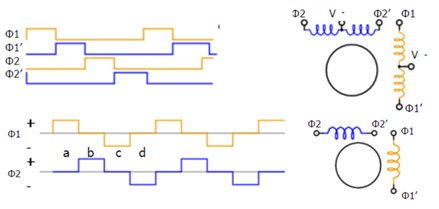
\includegraphics[scale = 1]{img/Picture9.png}
    \end{center}
\end{figure}

\begin{itemize}
    \item Řízení podle sekvence: \begin{itemize}
              \item Jednofázové řízení - wave-drive - vždy spínaná pouze jedna fáze (jedno vinutí)
              \item Dvoufázové - full nebo half step\begin{itemize}
                        \item Full step - vždy sepnuty dvě vinutí vedle sebe - pořád stejný moment, ale větší krok
                        \item Half step - Sepnuto jedno vinutí => sepnuta dvě vedle sebe => sepnuto druhé vinutí, menší krok (plynulejší), rozdílný moment v jednotlivých fázích.
                        \item Microstepping - Postupné buzení jednotlivých kroků
                    \end{itemize}
              \item Řízení driverem: \begin{itemize}
                        \item Ovládání nadřazeným systémem - step, driv, enable sígnály
                        \item S nadřazeným systémem komunikuje po sběrnici - EtherCAT, Profinet, SPI,\dots
                    \end{itemize}
          \end{itemize}
\end{itemize}

\subsubsection*{Výhody a nevýhody krokových notorů}
\begin{itemize}
    \item Výhody: \begin{itemize}
              \item Polohování v otevřené smyčce
              \item Přesné polohování, velký moment
              \item Rychlost nezávisí na zátěži, konstantní příkon
              \item Více možností zapojení, snadné přepínání fází
          \end{itemize}
    \item Nevýhody: \begin{itemize}
              \item nízká rychlost
              \item Rezonance - vibrace, hluk
          \end{itemize}
    \item Oproti servo-pohonům jsou levnější, jednodušší, momentově silnější při stejné rychlosti, méně přesné, pomalejší, méně dynamické.
\end{itemize}

\subsubsection*{Servopohon}
Řízení krokového motoru v uzavřené smyčce může určit fázový přechod s polohou rotoru pomocí zpětné vazby polohy a (nebo) zpětné vazby rychlosti, což může výrazně zlepšit výkon krokového motoru. -> servopohony
\begin{itemize}
    \item motor + zpětná vazba + regulátor
    \item drahé, složitá elektronika, řízení komunikací
\end{itemize}

\subsubsection*{Asynchronní motor}
\begin{itemize}
    \item Napájen střídavým 3-fázovým napětím
    \item Zapojení do hvězdy(výkon) nebo trojuhelníka (proud)
    \item Staror - cívky, Rotor - klec z feromagnetického materiálu
    \item Levný, odolný proti přetížení, nejrozšířenější druh motoru
    \item Velký počáteční proud, složité na řízení na polohu
    \item Má skluz - tok magnetického pole je rychlejší než otáčení rotoru
    \item Reverzace směru otáčení - prohození fází
\end{itemize}

\subsubsection*{Řízení}
\begin{itemize}
    \item Pomocí stykače (el. signálem)
    \item Pomocí frekvečního měniče - elektrické signály (start/stop, forward/reverse,\dots), pomocí komunikace (registry)
    \item Řízení rychlosti - napětím, frekvencí
\end{itemize}

\subsubsection*{Synchronní motor - PMSM}
\begin{itemize}
    \item Napájen střídavým 3-fázovým napětím
    \item Stator - cívky, Rotor - magnet (podoba s BLDC)
    \item Neumí se sám rozběhnout - přidává se např. klec z feromagnetika jako u indukčního
    \item Dražší, přesnější, nemá skluz
    \item Lepší řízení na polohu než asynchronní.
\end{itemize}

\subsection{Pneumatické pohony}
\subsubsection*{Fyzikální podstata}

\begin{figure}[h]
    \begin{center}
        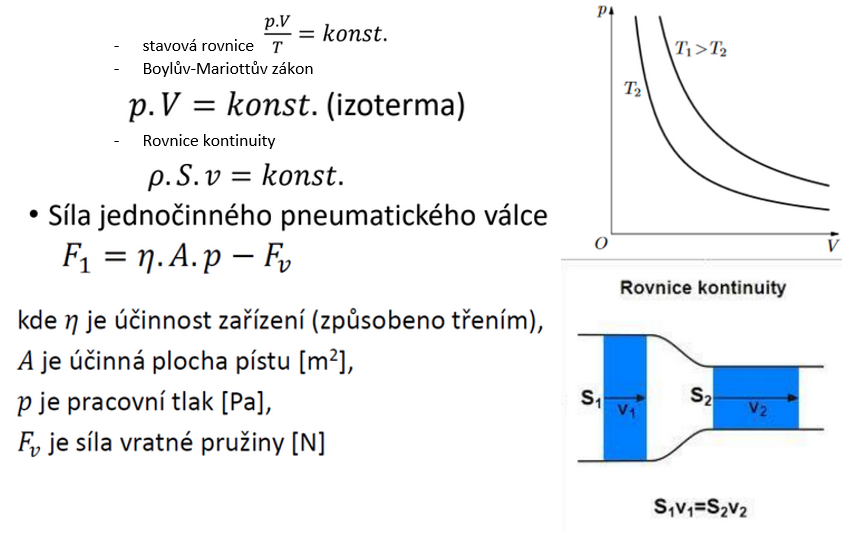
\includegraphics[scale = 0.7]{img/Picture12.png}
    \end{center}
\end{figure}

\begin{itemize}
    \item Komponenty: \begin{itemize}
              \item lineární - pneumatický válec
              \item rotační - rotační pneumatický pohon
              \item kyvný - kyvný pneumatický pohon
          \end{itemize}
    \item Přeměnu pneumatické tlakové energie na mechanickou zajišťuje: \begin{itemize}
              \item membrána
              \item píst (piston)
              \item vlnovcelamely
              \item lopatky - turbína
          \end{itemize}
\end{itemize}

\begin{figure}[h]
    \begin{center}
        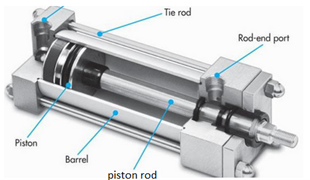
\includegraphics[scale = 1]{img/Picture10.png}
    \end{center}
\end{figure}

\subsubsection*{Vlastnosti}
\begin{itemize}
    \item Dostupnost - Stalčený vzduch je ve většině podniků k dispozici, případně pojízdné kompresory
    \item Skladování - Velké objemy stlačeného vzduchu lze skladovat
    \item Jednoduchá konstrukce - Pneumatické prvky mají jednoduchou konstrukci
    \item Řízení proudu a tlaku - Lze dobře nastvovat pomocí škrtícího ventilu
    \item Trvanlivost při malých nárocích na údržbu
    \item Bez negativních vlivů na životní prostředí
    \item Bezpečnost - pneumatické pohony se při provozu nezahřávají, při přetížení se zastaví a nepoškodí se
\end{itemize}

\subsubsection*{Výhody}
\begin{itemize}
    \item Možnost rozvodu a delší vzdálenost
    \item Rychlé pohyby
    \item Snadná regulace a automatizace
    \item Vzduch je dostupné a bezpečné médium
    \item Cenová dostupnost komponent
\end{itemize}

\subsubsection*{Nevýhody}
\begin{itemize}
    \item Omezená síla
    \item Problematické dosažení pomalých či plynulých pohybů
    \item Nutná úprava vzduch
    \item V důsledku špatné údržby vznikají netěsnosti
    \item Hlučné, Nelinearita, je třeba mazat (bezolejové provedení)
\end{itemize}

\section{Řídicí členy (PLC, DCS, průmyslová PC, průmyslové regulátory, vestavné systémy, HMI aj.) – vlastnosti a použití. Typy provedení komponentů. Možnosti jejich programování (parametrizace, reprezentace veličin, struktura projektu, struktura programu, stavový automat). Postup programování technologických procesů.}

\subsection{Reléová Logika}
Realizování logiky pomocí soustav relátek. Dříve tak muselo být realizováno vše, dnes už max jen jednoduché zapojení. Nahrazeno logikou v PLC.

\subsection{PLC}
\begin{itemize}
    \item Malý průmyslový počítač pracující v reálném čase.
    \item Je u něj kladen velký důraz na spolehlivost - z toho důvodu jsou používány procesory, které jsou již ověřené (Chybovost atp.).
    \item Nasazován pro řízení strojů, výrobních linek, robotů, sběr dat ze zařízení atp.
    \item Zpravidla obsahuje rozhraní pro komunikaci - sériová linka, ethernetové porty, USB (k programování).
    \item Většinou má digitální a analogové vstupy/výstupy.
    \item Programuje se dle standardu IEC 61131 - jazyky Structured Text, Ladder, Function Block Diagram,\dots
    \item Programuje se ve vývojovém prostředí - každý výrobce používá většinou to své, např. Siemens - TIA portal. Případně se často využívá CODESYS.
\end{itemize}
\subsubsection*{Struktura PLC}
\begin{itemize}
    \item Vnější: \begin{itemize}
              \item Zdroj
              \item Procesor
              \item IO moduly
              \item Komunikační moduly
          \end{itemize}
    \item Vnitřní: \begin{itemize}
              \item Napájecí modul
              \item Vstupní modul
              \item Procesorová jednotka
              \item Paměť pro data
              \item Paměť pro program
              \item Výstupní model
          \end{itemize}
\end{itemize}

\begin{figure}[h]
    \begin{center}
        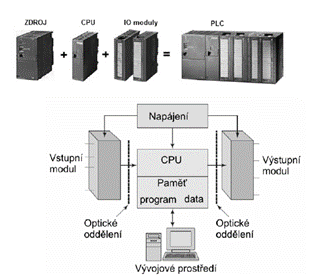
\includegraphics[scale = 1]{img/Picture13.png}
    \end{center}
\end{figure}

\subsubsection*{Konstrukce}
\begin{itemize}
    \item Kompaktní - jednodušší, všechny vnější komponenty jsou v jedné "krabičce"
    \item Modulární - větší, dražší, viz obrázek
\end{itemize}

\subsubsection*{Komunikační rozhraní}
\begin{itemize}
    \item Point to point - programování
    \item Multi point interface - programování a jednoduchá komunikace
    \item Čím dál častěji se využívají komunikační protokoly přes ethernet - Ethernet/IP, ProfiNET, Modbus TCP, EtherCAT,\dots
    \item Případně komunikace přes RS422, RS 485, Profibus,\dots
\end{itemize}

\subsubsection*{Programovatelné relé}
Miniaturní PLC s omezenými možnostmi (výkon, komunikace, IO). Integruje několik relé, časovačů a jednoduchou komunikaci.

\subsubsection*{Soft PLC}
Celé zařízení vykonává standardní PC, případně umí i Raspberry Pi, ve kterém je nainstalován software, který emuluje PLC. Připojení různých rozhraní je pomocí modulů, které jsou připojeny k PC.
\begin{itemize}
    \item Levnější
    \item Velká operační paměť
    \item Není až tak moc realtime kvůli operačnímu systému.
\end{itemize}

\subsubsection*{Slot PLC}
PLC realizováno jako karta do PC

\subsubsection*{Průmyslový počítač - IPC}
\begin{itemize}
    \item Je to počítač přizpůsoben do průmyslového prostředí.
    \item Má pasivní chlazení, vysoká tepelná odolnost, dlouhá životnost, spolehlivost, ochrana proti prachu, mechanická odolnost.
    \item Operační systém - Windows embedded, Linux RT, RTX.
    \item Z hlediska průmyslového řízení má několikanásobně vyšší výkon než PLC.
    \item Oproti PLC jsou zaměřeny spíše na komunikace než na IO.
    \item Spíše starší HW - starší HW je více otestován na krizové situace.
\end{itemize}

\subsubsection*{Procesní stanice}
\begin{itemize}
    \item Rozšiřuje řídící komponentu o IO.
    \item U modernějších typů možná i parametrizace.
    \item Ovládaná pomocí průmyslové komunikace.
    \item Jsou velké - i 150 IO.
    \item Nemá logiku, jen vykonává příkazy
\end{itemize}

\subsubsection*{DCS}
\begin{itemize}
    \item DCS = Distributed Control System.
    \item Každá řídící komponenta má na starost svou dílčí oblast, která je do jisté míry autonomní - například PLC.
    \item Tyto komponenty komunikují mezi sebou, případně s nadřazeným systémem, který je ovládá jako celek.
\end{itemize}

\subsubsection*{HMI}
\begin{itemize}
    \item HMI = Human Machine Interface.
    \item Rozhraní mezi člověkem a strojem, vizualizace a řízení menších technologických celků (stroj, linka,\dots).
    \item Nepodporuje realtime OS.
    \item Integrován jako HMI panel zabudován ve stroji, HMI+PLC dohromady (Když se jedno posere, musí se vyměnit celek).
    \item Propojení pomocí průmyslové komunikace - ethernet - Modbus TCP, Ethernet/IP, \dots
    \item HMI může být využíváno pro konkretní stroj nebo jako jedno HMI na více strojů - více obrazovek.
\end{itemize}

\subsubsection*{Průmyslové regulátory}
\begin{itemize}
    \item Jednoúčelová komponenta pro regulaci nějakého procesu na základě vstupu. Např. pro regulaci teploty.
    \item Pravděpodobně vždy PID regulátor. Většinou má auto-tuning (Automatické určení regulované soustavy).
\end{itemize}

\subsubsection*{Vestavné systémy}
Tak tu fakt nevim, co po nás z "PPA gangu" chcou - bude to chtít naučit se i BPC-MIC :)

\subsubsection*{Programování dle IEC61131}
Parametrizace a programování PLC se dnes už často dělá dle této normy

\begin{figure}[h]
    \begin{center}
        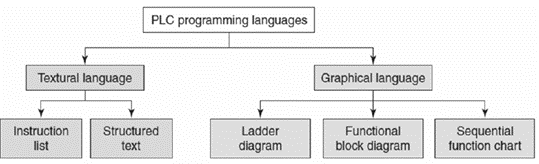
\includegraphics[scale = 1]{img/Picture14.png}
    \end{center}
\end{figure}

\begin{itemize}
    \item Zdrojový kód se pak píše do \textbf{Program Organisation Unit (POU)}, což může být funkce, funkční blok, nebo kus programu.
    \item Tyto POU pak mohou být zařazeny do \textbf{Task}ů. Každý Task má pak definován, jak často je vykonáván – periodicky, při události, v každém cyklu PLC.
    \item Dle normy je taky oddělená konfigurace PLC a modulů a definice CPU (Resource), který vykonává Tasky.
    \item Každý projekt může mít několik seznamů globálních proměnných, pomocí kterých mohou POU mezi sebou komunikovat.
\end{itemize}

Tato norma také definuje jakým způsobem pracuje PLC. Pracuje v tzv. cyklech, kdy dokola provádí následující operace:
\begin{itemize}
    \item Čtení stavů vstupů do vnitřní paměti
    \item Vykonání celého programového vybavení pracujícího s vnitřní pamětí
    \item Zpracování komunikace
    \item Diagnostika chybovosti
    \item Zápis stavů výstupů z vnitřní paměti
\end{itemize}

\subsubsection*{Task}
\begin{itemize}
    \item Sbírka podprogramů vykonávající se v daném pořadí - najednou.
    \item Kontinuální task - vykonává se vždy, když je to možné - přerušení s periodickým taskem
    \item Periodický task - spoušten v daný okamžik s periodou
    \item Událostní task - spouštěn na zákaldě splnění nějaké podmínky
\end{itemize}

\subsubsection*{Vestavěné funkce}
\begin{figure}[h]
    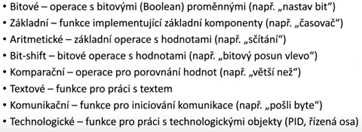
\includegraphics[scale = 0.85]{img/Picture15.png}
\end{figure}

\subsubsection*{Datové typy}
\begin{figure}[!h]
    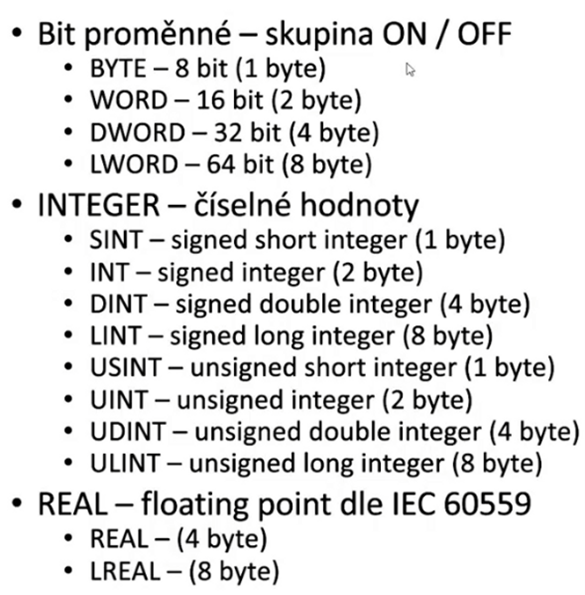
\includegraphics[scale = 0.85]{img/Picture16.png}
\end{figure}

\subsubsection*{Postup pro vytvoření programu}
\begin{itemize}
    \item HW konfigurace
    \item Konfigurace komunikace
    \item Vytvoření seznamu aliasů (GVL)
    \item Vytvoření programu
    \item Nahrání do PLC a testování
\end{itemize}

\subsubsection*{Režimy PLC}
\begin{itemize}
    \item STOP - výstupy neaktivní, vstupy Aktivní
    \item RUN
    \item ERROR
    \item MAINT - režim údržby
\end{itemize}

\subsubsection*{Postup programování technologických procesů}
\begin{itemize}
    \item Model logického programu \begin{itemize}
              \item Nastavování výstupů na základě časových a logických podmínek
              \item Jednoduchý a názorný přístup
              \item Nutno úplně definovat podmínky nastavování
          \end{itemize}
    \item Model sekvenčního programu \begin{itemize}
              \item Nastavování výstupu na základě stavu programu
              \item Systematický přístup
              \item Úloha rozdělna na posloupnost kroků
              \item např. stavový automat
          \end{itemize}
\end{itemize}

\subsubsection*{Stavový automat}
Viz BPC-LOS - Mealy, Moore

\section{Průmyslové komunikační sítě (sběrnice a protokoly) – dělení, vlastnosti a použití. Referenční model ISO/OSI. Způsoby komunikace. Průmyslový Ethernet. Bezdrátový přenos dat v průmyslovém prostředí.}
\subsubsection*{Referenční model ISO / OSI}
Tento model popisuje chování klientů při komunikaci, definuje služby, protokoly a rozhraní pro jednotlivé vrstvy.
\begin{itemize}
    \item 7. Aplikační vstva - rozhraní na aplikaci (nebo OS)
    \item 6. Prezentační vrstva - konverze dat, šifrování, komprese
    \item 5. Relační vrstva - ustanovení relace, autorizace, autentizace [data]
    \item 4. Transportní vrstva - řízení toku dat přes síť [segment]
    \item 3. Síťová vrstva - směrování, adresování, udržování síťových spojení [paket]
    \item 2. Spojová vrstva - zajišťuje spojení bod-bod (oprava chyb, adresování, rámce, tok, přístup k médiu) [rámec]
    \item 1. Fyzická vrstva - fyzické parametry komunikace (specifikace HW, el. signály, konektory, vedení) [bit]
\end{itemize}

\subsubsection*{Fyzická vrsta ISO/OSI}
Rozlišujeme několik typů zpaojení týkajících se fyzické vstvy ISO/OSI modelu:
\begin{itemize}
    \item Nesymetrický přenos - Signál vztahován k zemi, jednoduchý, levný, málo odolný protio rušení, krátká vzdálenost, malá rychlost
    \item Symetrický přenos - Signály vztahovány proti sobě, měří se potenciál mezi dvěma vodiči. Vysoké rychlosti, velká odolnost vůči rušení.
    \item Point-to-Point (simplex) - 1 vysílač, 1 přijímač - komunikace v jednom směru
    \item Multidrop (distributed simplex) - 1 vysílač, více přijímačů - komunikace v jednom směru
    \item Multipoint (mupliplex) - více vysílačů i přijimačů, obousměrná komunikace
    \item Half-Duplex - obousměrná komunikace - v jeden okamžik pouze v jednom směru
    \item Full-Duplex - obousměrná komunikace - v obou směrech najednou
\end{itemize}

\subsubsection*{Spojová vrsva ISO/OSI}
Přenos a synchronizace rámců, řízení toku, detekce a ošetření chyb. U ethernetu například switche - pomocí MAC adresy směřují rámce na správné porty.

\subsubsection*{Síťová vrstva}
Slouží ke konkrétnějšímu směrování rámců. Rozlišuje se několik druhů adresování:
\begin{itemize}
    \item Unicast - zpráva pro jediného příjemce
    \item Anycast - zpráva pro příjemce v určitém dosahu
    \item Multicast - zpráva pro skupinu příjemců
    \item Broadcast - zpráva určená všem
\end{itemize}
S touto vrstvou pracují například routery, které podle IP adresy směřují pakety na správné zařízení.

\subsubsection*{Průmyslové komunikační sítě - protokoly}
Používají se pro přenos dat ve větším množství, nebo pokud chceme připojovat více zařízení na stejnou sběrnici.
Rozděluje se do několika kategorií (od nejjedodušší k nejsložitější):
\begin{itemize}
    \item \textbf{Sensor Bus} - K propojení senzorů s řídícími systémy. AS-interface, IO-Link
    \item \textbf{Device Bus} - K propojení zařízení jako akční prvky (ventily, motory,...) s řídícími systémy. Profibus DP, CANopen\dots
    \item \textbf{Fieldbus} - K propojení senzorů, akčních prvků a dalších průmyslových zařízení se řídícími systémy. Profibus PA, Modbus,\dots
    \item \textbf{Průmyslový ethernet} - Využití výhod ethernetu s kombinací prvků z průmyslu. Ethernet/IP, Modbus TCP, Profinet, Powerlink, EtherCAT\dots
\end{itemize}

\begin{figure}[h]
    \begin{center}
        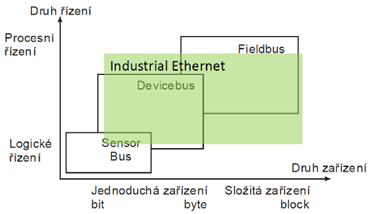
\includegraphics[scale = 1]{img/Picture17.png}
    \end{center}
\end{figure}

\begin{figure}[!h]
    \begin{center}
        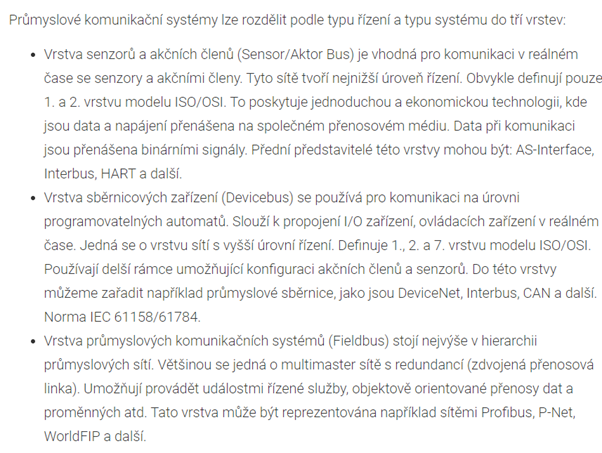
\includegraphics[scale = 1]{img/Picture18.png}
    \end{center}
\end{figure}

\newpage

\subsubsection*{AS-Interface}
\begin{itemize}
    \item Sensor Bus
    \item Různé topologie, plug and play
    \item Speciální fyzická vrstva s profilovým nestíněným nekrouceným kabelem
    \item Především pro přenos binárních signálů (0,1)
    \item Jen do nevýbušného prostředí, existuje i varianta pro toto prostředí.
\end{itemize}

\subsubsection*{Profibus}

\begin{itemize}
    \item V průmyslu je stále nejrozšířenějším protokolem
    \item Profibus DP (decentralized periphery) - devicebus - rychlejší, jednodušší, využívá RS-485, optika. Optimalizován na výkon, cyklický přenos dat
    \item Profibus PA (process automation) - fielbus - pomalejší, bezpečnější (aj výbušné prostředí), využívá vlastní fyzickou vrstvu.
    \item Profibus využívá deterministickou komunikaci v reálném čase.
\end{itemize}

\subsubsection*{HART}
\begin{itemize}
    \item Sériový protokol umožňující digitální přenos příkazů přes analogovou proudovou smyčku 4-20mA pomocí změn frekvence
    \item Umožňuje diagnostiku, seřizování a parametrizaci přístrojů
    \item Existuje i bezdrátová varianta - WirelessHART
\end{itemize}

\subsubsection*{Průmyslový ethernet}
Postupnou konvergencí průmyslu k internetu jsme dospěli k tomu, že je velmi praktické jako fieldbus používat ethernet. Dostaneme tak řešení, které je mnohem více standardizované, rychlejší, lze využít mnoho poznatků z provozování běžných sítí (např. rozdělování přístupu) a lze na něm provozovat i „běžné“ počítačové komunikace.
Je u něj třeba zaručit několik real-time vlastností:
\begin{itemize}
    \item Včasnost - rychlost provedení operace od vyslání zprávy - zajistí se fyzickým oddělením časově kritické komunikace od časově nekritické, nebo třeba prioritizací paketů na úronvi switchů
    \item Současnost - synchronizace akcí všech účastníků na ethernetu - zajistí se mechanismy na synchronizaci času - časové značky u paketů
\end{itemize}
Další z možností jak tyto dvě vlastnosti zařídit: Použít UDP namísto TCP, snížit časové toleranční pásmo (jitter).

\begin{figure}[h]
    \begin{center}
        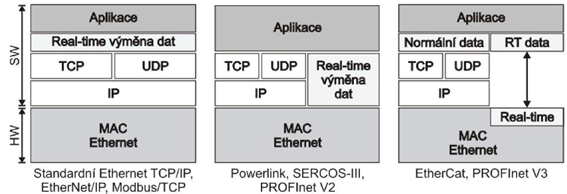
\includegraphics[scale = 1]{img/Picture19.png}
    \end{center}
\end{figure}

\subsubsection*{Modbus}
\begin{itemize}
    \item De facto standard pro průmyslové PLC komunikace
    \item Jednoduchá a rychlá digitální komunikace - Klient-Server
    \item Modbus RTU - sériové rozhraní (RS-485) (Fieldbus)
    \item Modbus TCP - průmyslový ethernet - datová část na TCP paketu (Průmyslový ethernet)
    \item Strikně Master-Slave protokol
\end{itemize}

\subsubsection*{Ethernet/IP}
\begin{itemize}
    \item Ethernet industrial protocol
    \item Časově kritické zprávy přenášeny způsobem producent-konzument
    \item Konfigurace a parametry přes TCP
    \item Časově kritické data přes UDP
\end{itemize}

\subsubsection*{Profinet}
\begin{itemize}
    \item Návaznost na profibus, redundantní topologie a safety funkce.
    \item Profinet CBA - TCP/IP komunikace, jitter 5-100 ms, cyklus sítě nad 100 ms
    \item Profinet IO-RT - decentralizované periferie, především cyklický režim, jak profibus DP, jitter 10-100 us, cyklus sítě 5-10 ms
    \item Profinet IO -IRT - real-time cyklická komunikace se servoměniči, spešl HW, jitter 1-100 us, cyklus sítě 31,25us - 1ms
\end{itemize}

Ještě tu je aj \textbf{EtherCAT} a \textbf{ETHERNET Powerlink}, ale na ty kukněte do prezentace, ať jen víte, že existují\dots

\subsubsection*{Bezdrátová komunikace}
\begin{itemize}
    \item Rádiové vlny - elektromagnetický signál v rozsahu 3 kHz až 300 GHz \begin{itemize}
              \item Analogová modulace (AM,FM,\dots)
              \item Digitální (ASK,FSK,GSk,\dots)
          \end{itemize}
    \item Síla signálu se vyjadřuje jako výkon [W].
\end{itemize}

\subsubsection*{Bezdrávoté technologie}
\begin{itemize}
    \item Wireless MAN (metropolitní síť) \begin{itemize}
              \item WiMAX, GPRS, EDGE, UMTS, HSDPA,\dots
          \end{itemize}
    \item Wireless LAN (lokální sítě) \begin{itemize}
              \item Wi-Fi, HIPERLAN, DECT,\dots
          \end{itemize}
    \item Wireless PAN ("osobní" sítě (krátkého dosahu)) \begin{itemize}
              \item Bluetooth, ZigBee, WirelessHART,\dots
          \end{itemize}
\end{itemize}

\section{Spolehlivost a bezpečnost průmyslových zařízení a systémů. Metody vyhodnocení spolehlivosti. Komponenty a metody zajišťující funkční bezpečnost průmyslových strojů a zařízení. Aspekty kybernetické bezpečnosti. Kybernetické útoky a metody jejich zmírnění.}

\subsubsection*{Definice spolehlivosti a bezpečnosti}
Čeština má jedno slovo pro slovo SAFETY a SECURITY = Bezpečnost.
\begin{itemize}
    \item \textbf{Safety} - bezpečnost při práci a funkční bezpečnost výrobních zařízení
    \item \textbf{Security} - datová bezpečnost a kyberbezpečnost
    \item \textbf{Spolehlivost} - schopnost systému plnit danou funkci v daném časovém intervalu
\end{itemize}

\subsubsection*{Riziko a jeho vyhodnocení}
\begin{itemize}
    \item Riziko = Pravděpodobnost újmy * Závažnost následku
    \item Pravděpodobnost újmy = frekvence poškození za rok
    \item Závažnost následku - peněžní, lidské
    \item Proces je považován za bezpečný, pokud je množství vznikající újmy na zdraví, poškození životního prostředí a poškození produkce během procesu akceptovatelný.
    \item Maximální přijatelné riziko si definujeme tím, kam umístíme červenou čáru\dots
\end{itemize}

\begin{figure}[h]
    \begin{center}
        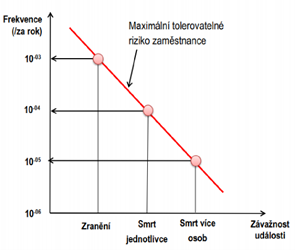
\includegraphics[scale = 1]{img/Picture20.png}
    \end{center}
\end{figure}

\begin{itemize}
    \item \textbf{Bezpečnost} - souhrn úkolů pro odstranění nepřijatelného rizika
    \item \textbf{Bezpečností funkce (SIF)} - funkce, kterou systém realizuje pro snížení rizika
    \item \textbf{Intenzita poruch} - očekávaný počet nezávislých poruch za jednotku času
    \item \textbf{MTBF} - střední doba mezi poruchami
    \item \textbf{MTTF} - středí doba do poruchy
\end{itemize}

\subsubsection*{Koncepce SIL}
Čím větší redukce rizika je vyžadována, tím vyšší je SIL bezpečností funkce. => definuje požadavky na bezpečnostní funkce (SIF) zařízení.
\begin{itemize}
    \item Safety Integrity Level je odstupňovaný soubor opatření určený ke snížení rizika na tolerovatelnou úroveň.
    \item Požaduje splnění požadavků - kvantitativní požadavky na minimální hladinu redundance (tolerance k chybám HW, podíl bezpečných a nebezpečných poruch), Kvalitativní požadavky (Vhodnost komponentů, požadavky pro SWm,\dots)
    \item \textbf{Integrita bezpečnosti} - pravděpodobnost, s jakou bude bezpečnostní systém uspokojivě plnit požadované bezpečnostní funkce za všech podmínek po stanovenou dobu.
    \item Probability of failure per demand (PFD) - pro "low demand" systémy
    \item Probability of failure per hour (PFH) - pro "high demand" systémy
\end{itemize}

\subsubsection*{Funkční Bezpečnost - životní cyklus provedení bezpečnostních opatření stroje}
\begin{itemize}
    \item \textbf{Identifikace rizik}: Nejdůležitějším prvním krokem je identifikace všech rizik spojených s daným strojem. Tyto rizika mohou být fyzická, elektrická, chemická nebo jiné povahy.
    \item \textbf{Analýza rizik}: Po identifikaci rizik se provádí jejich analýza, aby se posoudila vážnost a pravděpodobnost každého z nich a určilo se, jaká bezpečnostní opatření jsou nezbytná k minimalizaci rizik.
    \item \textbf{Návrh bezpečnostních opatření}: Na základě výsledků analýzy rizik se navrhují a implementují vhodná bezpečnostní opatření. Tyto opatření mohou být fyzické, jako jsou například bariéry nebo zábrany, nebo technické, jako jsou například senzory nebo automatické vypínání.
    \item \textbf{Testování a ověření}: Po implementaci bezpečnostních opatření se provádí testování, aby se zajistilo, že jsou opatření účinná a odpovídají požadovaným bezpečnostním standardům.
    \item \textbf{Monitorování a údržba}: Bezpečnostní opatření musí být pravidelně monitorována a údržbou, aby bylo zajištěno, že zůstávají účinná a nezhoršují se. Také je důležité průběžně sledovat a aktualizovat bezpečnostní opatření v případě, že se změní podmínky provozu stroje nebo změní bezpečnostní standardy.
    \item \textbf{Odstranění stroje}: Nakonec, když je stroj starý nebo již není bezpečný, musí být odstraněn v souladu s příslušnými normami a zákony.
\end{itemize}
(převzato z BPC-PGA - lepší popis než z obrázku - obsahuje ještě 6. část, kdy se stroj odstraní)

\begin{figure}[h]
    \begin{center}
        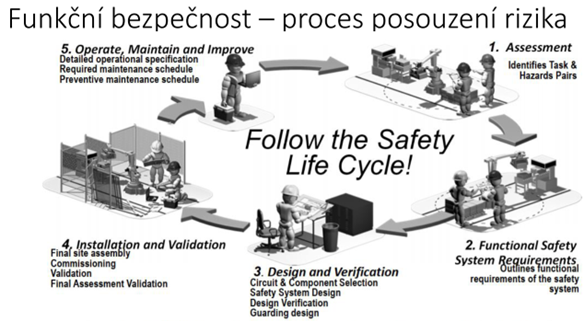
\includegraphics[scale = 1]{img/Picture21.png}
    \end{center}
\end{figure}

\subsubsection*{Funkční bezpečnost - metody boje proti chybám}
\begin{itemize}
    \item Predcházení chybám (Fault prevention, avoidance): \begin{itemize}
              \item Konstrokční chyby - upravení procesu, řízení kvality,\dots
              \item Provozní chyby - stínění, vhodné podmínky,\dots
          \end{itemize}
    \item Odstranění chyb (fault removal) \begin{itemize}
              \item Verifikace a validace - při návrhu, kontrola, analýza,\dots
              \item Údržba - při provozu, mazání, pravidelná kontrola,\dots
              \item Fault forecasting - simulace, modelování, historuická data, testy,\dots
          \end{itemize}
    \item Maskování chyb (fault masking) \begin{itemize}
              \item Zabránění projevu chyby - redundance (2 zařízení dělaj to samé, při chybě začne fungovat druhé)
          \end{itemize}
    \item Odolnost proti chybám (fault tolerance) \begin{itemize}
              \item Detekce chyby (fault detectino) - watchdog (periodický občerstvovaný časovač - monitoruje a reaguje na problémy)
              \item Zotavení (recovery) - restart
              \item Odstranění poruchy (fault removal) - načtení naposledy správného stavu
          \end{itemize}
\end{itemize}

\subsubsection*{HW funkční bezpečnost}
\begin{itemize}
    \item Vstupy - STOP tlačítko, světelná závora, zámek, koncový spínač, ruční spínač (deadman switch)
    \item Výstupy - Bezpečnostní stykače, frekvenční měniče s bezpečnostními funkcemi,\dots
    \item Logické obvody - Bezpečnostní relé, safety PLC,\dots
\end{itemize}

\subsubsection*{Chyby - pojmy}
TIP - nauč se hlavně anglický pojem, čeština je mrcha. A i tak v tom budeš mít guláš
\begin{itemize}
    \item Fault (závada,chyba) - defekt, potenciální příčina chyby systému
    \item Error (chyba, porucha) - nesprávný stav systému, může vést k selhání
    \item Failure (porucha, selhání) - defekt, systém neplní požadovanou funkci
    \item Havárie - porucha s vážnými následky
    \item Fault tolerance (odolnost proti poruchám) - závada nevede k poruče
    \item Safety (bezpečnost) - porucha nevede k havárii
\end{itemize}

\subsubsection*{Ukazatele spolehlivosti}

\begin{itemize}
    \item Intenzita poruch - očekavaný počet poruch za jednotku času - počet poruch za milion provozních hoditn nebo jako Failure in time (miliarda hodin)
    \item Střední doba bezporuchového provozu (MTBF) - střední doba mezi dvěma poruchami
    \item Střední doba do poruchy (MTTF) - nezahrnuje dobu opravy, rozlišení poruchy a nebezpečné poruchy
\end{itemize}

\begin{figure}[h]
    \begin{center}
        \includegraphics[width = \textwidth]{img/Picture23.png}
    \end{center}
\end{figure}

\subsubsection*{Analýza spolehlivosti}
\begin{itemize}
    \item Analýza stromu poruchových stavů (FTA) - postup shoda dolů, hledání možných příčin jednotlivých poruchových stavů, zápis formou diagramu
    \item Failure mode and effects analysis (FMEA) - postup shora nahoru, hledání možných poruch a jejich vlivu na fungování systému, posouzení závažnosti poruch, četnosti, možnost odhalení,\dots Zápis formou tabulky.
\end{itemize}

\subsubsection*{Kybebezpečnost v průmyslu}
Je třeba zajistit zabezpečení dat v celém podnikovém systému – celistvost a nepodvrhnutelnost dat, bezpečný přenos dat, zabezpečení před neoprávněnou manipulací.
\begin{itemize}
    \item Vnější aspekty - ochrana před útočníky z vnějšku
    \item Vnitřní aspekty - Ochrana přes samotnými zařízeními a nedbalostí zaměstanců
\end{itemize}

\subsubsection*{Zranitelná místa a útoky}
\begin{itemize}
    \item Backdoor - neúmyslně při návrhu nebo konfiguraci, případně úmyslně
    \item Denial of Serivce (DoS) - znemožnění dostupnosti síťové služby
    \item Útok s přímým přístupem - červ, keylogger, trojan, ransomware,\dots
    \item Odposlech - odcizení firemních informací
    \item Spoofing - podvrhnutí dat vedoucí k poškození procesů ve výrobě
    \item Tampering - modifikace zařízení pro získání dozoru, "Evil made attack"
    \item Phising - snaha získat citlivé informace, sociální inženýrství
\end{itemize}

\subsubsection*{Zamezení kybernetickým útokům}
\begin{itemize}
    \item Bounty program - finanční kompenzace za nalezení chyb, aby tyto chyby nebyly prodány zlé straně
    \item Zabezpečení fyzického přístupu - autorizace, autentizace
    \item Zabezpečení IT systému - VLAN, Firewall, VPN, antiviry
    \item Zabezpečení informací - zálohování, šifrování dat
\end{itemize}

\subsubsection*{Prostředky pro kyberbezpečnost}
\begin{itemize}
    \item Zálohovací severy, HW šifrovací klíče, přístupové čipy, biometrika, kamerové systémy,\dots
\end{itemize}

\section{Systémy reálného času – vlastnosti a použití v průmyslové automatizaci. Pojmy determinismus, včasnost a jitter. Metody zajištění determinismu.}
Všechny systémy, které musí reagovat v reálném čase = musí vykonat akční zásah v reakci na podměty maximálně v definovaném čase.
\begin{itemize}
    \item Jde o všechny PLC, IPC zpracovávající časově-kritická data používané v průmyslu.
    \item Příklad real-time zpracování jsou například PLC dle IEC 61131, které podporují periodické a kontinuální úlohy. Kontinuální úlohy vykonává v každém cyklu PLC, periodické vždy jednou za nějaký časový úsek. Pokud je čas vykonat periodickou úlohu, pozastaví se vykonávání kontinuální úlohy a vykoná se periodická. Tohle „režíruje“ firmware PLC.
\end{itemize}

\subsubsection*{Determinismus, včasnost, jitter}
\begin{itemize}
    \item \textbf{Determinismus} - "opakovatelnost" událostí v systému. Deterministicky se chová něco, co se nechová náhodně, ale na základě jasných vstupů. V RTOS se tímto pojmem označuje to, že existují jasné časové meze při vykonávání funkce.
    \item  \textbf{Včasnost} - Požadavek na včasnost znamená, že vstupní data musejí být získána v časovém limitu. V tomto limitu musí být proveden výpočet a výstupní data musí být dýna na výsutp. Dá se posuzovat dvěma rúznými časovými podmínkami: \begin{itemize}
              \item Absolutní časová podmínka - V daný čas musí být podmínka splněna
              \item Relativní časová podmínka - Podmínka musí být splněna do x sekund od splnění jiné podmínky.
          \end{itemize}
    \item \textbf{Jitter} - Variabilita periodicity (nestálost frekvence) - velikost kolísání při odezvě internetu.
\end{itemize}

\begin{figure}[h]
    \begin{center}
        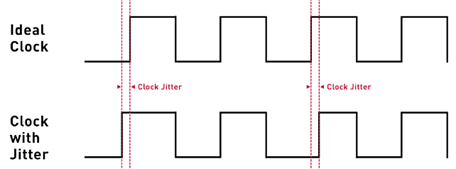
\includegraphics[scale = 1]{img/Picture24.png}
    \end{center}
\end{figure}

\subsubsection*{Řízení v supersmyčce}
Jednoduché, intuitivní řešení, vhodné pro jednoduché úlohy. Není potřeba žádná složitá režie – není potřeba operační systém. Složitější úlohy takhle nelze řešit, nebyly by real-time kvůli zpoždění.
Je definována jako situace kdy:
\begin{itemize}
    \item Úlohy jsou implementovány jako funkce
    \item Úlohy volány za sebou ve while cyklu
    \item Úlohy jsou řazeny za sebou
\end{itemize}
Problém s délkou cyklu nastane, když do cyklu zařadíme např. komunikace, nebo složitější úlohy.
Pokud potřebujeme přesnou periodu, musíme měřit čas a variabilní dobu na konci čekat.

\subsubsection*{Víceúlohové operační systémy}
\begin{itemize}
    \item Dekompozice úlohy na samostatné procesy vede ke zjednodušení procedur a ke snadnějšímu ladění/ověření jejich funkce.
    \item Selhání jednoho procesu nemusí nutně vést k selhání celého systému.
    \item Procesům lze různě přiřadit priority.
    \item Pararelismus se systémem priorit a deterministickým plánovačem jádra (kernel) je NUTNOU podmínkou pro real-time chování řídící úlohy
    \item Snadnější úpravy, možnost zaručení real-time odezvy, více složitý, režie OS
\end{itemize}

\subsubsection*{Operační systém reálného času (RTOS)}
\begin{itemize}
    \item takový OS, který je schopen provádět výpočy a reagovat na událost v definovaných časových intervaltech (v deadlines).
    \item Musí obsahovat deterministický plánovač jádra
    \item Podmínka realizace v RTOS není dostačující – programátor musí vždy řídicí úlohu přizpůsobit schopnostem a možnostem daného RTOS na dané HW platformě
\end{itemize}

\subsubsection*{Deadline}
\begin{itemize}
    \item Hard - požadavky musí být bezpodmínečně splněny při každé vyskytnuté události v systému
    \item Soft - stačí, když budou slněny v nějakém průměrném časovém intervalu
    \item V informatickém pojetí jsou v hard deadlines systémech data, která přijdou pozdě bezcenná, popřípadě neplatná a mnohdy i potenciálně nebezpečná. Systém s nimi často nesmí dále pracovat. Pokud by hard deadlines splněny nebyly, došlo by k selhání systému se všemi z toho vyplývajícími důsledky.
\end{itemize}
Má několik softwarových součástí:
\begin{itemize}
    \item 1. Správa úloh - vyhodnocuje a zařazuje úlohy
    \item 2. Správa paměti - alokuje a dealokuje paměť
    \item 3. Meziprocesorová komunikace - synchronizace úloh
    \item 4. Správa zařízení - drivery, HAL (Hardware Abstraction Layer)
    \item 5. Správa času - obnova časovačů, hlídání času
\end{itemize}

Příklady RTOS
\begin{itemize}
    \item POSIX (Linux) - QNX, LynxOS
    \item Win32 - Windows CE
    \item Embedded (ARM) - FreeRTOS
\end{itemize}

RTOS vs supersmyčka:
\begin{figure}[h]
    \begin{center}
        \includegraphics[width = \textwidth]{img/Picture25.png}
    \end{center}
\end{figure}

\begin{itemize}
    \item Aby mohly řídící prostředky pracovat v real time, musí obsahovat systém reaálného času - supersmyčka nebo RTOS
    \item RTOS je komplexní nástroj plnící deadline jednotlivých úloh
    \item RTOS se používá v PLC jako firmware, v embedded nebo PC řídících systémech
    \item Pro zajištění komunikace v real time je nutná součinnost software pracující v real time a HW.
\end{itemize}


